% Options for packages loaded elsewhere
\PassOptionsToPackage{unicode}{hyperref}
\PassOptionsToPackage{hyphens}{url}
%
\documentclass[
  english,
  man,floatsintext]{apa6}
\title{Infants' preference for speech is stable across the first year of life: Meta-analytic evidence}
\author{Cécile Issard\textsuperscript{1}, Sho Tsuji\textsuperscript{2}, \& Alejandrina Cristia\textsuperscript{1}}
\date{}

\usepackage{amsmath,amssymb}
\usepackage{lmodern}
\usepackage{iftex}
\ifPDFTeX
  \usepackage[T1]{fontenc}
  \usepackage[utf8]{inputenc}
  \usepackage{textcomp} % provide euro and other symbols
\else % if luatex or xetex
  \usepackage{unicode-math}
  \defaultfontfeatures{Scale=MatchLowercase}
  \defaultfontfeatures[\rmfamily]{Ligatures=TeX,Scale=1}
\fi
% Use upquote if available, for straight quotes in verbatim environments
\IfFileExists{upquote.sty}{\usepackage{upquote}}{}
\IfFileExists{microtype.sty}{% use microtype if available
  \usepackage[]{microtype}
  \UseMicrotypeSet[protrusion]{basicmath} % disable protrusion for tt fonts
}{}
\makeatletter
\@ifundefined{KOMAClassName}{% if non-KOMA class
  \IfFileExists{parskip.sty}{%
    \usepackage{parskip}
  }{% else
    \setlength{\parindent}{0pt}
    \setlength{\parskip}{6pt plus 2pt minus 1pt}}
}{% if KOMA class
  \KOMAoptions{parskip=half}}
\makeatother
\usepackage{xcolor}
\IfFileExists{xurl.sty}{\usepackage{xurl}}{} % add URL line breaks if available
\IfFileExists{bookmark.sty}{\usepackage{bookmark}}{\usepackage{hyperref}}
\hypersetup{
  pdftitle={Infants' preference for speech is stable across the first year of life: Meta-analytic evidence},
  pdfauthor={Cécile Issard1, Sho Tsuji2, \& Alejandrina Cristia1},
  pdflang={en-EN},
  pdfkeywords={Meta-analysis, Infants, Speech preference, Conspecific detection, Developmental tuning},
  hidelinks,
  pdfcreator={LaTeX via pandoc}}
\urlstyle{same} % disable monospaced font for URLs
\usepackage{graphicx}
\makeatletter
\def\maxwidth{\ifdim\Gin@nat@width>\linewidth\linewidth\else\Gin@nat@width\fi}
\def\maxheight{\ifdim\Gin@nat@height>\textheight\textheight\else\Gin@nat@height\fi}
\makeatother
% Scale images if necessary, so that they will not overflow the page
% margins by default, and it is still possible to overwrite the defaults
% using explicit options in \includegraphics[width, height, ...]{}
\setkeys{Gin}{width=\maxwidth,height=\maxheight,keepaspectratio}
% Set default figure placement to htbp
\makeatletter
\def\fps@figure{htbp}
\makeatother
\setlength{\emergencystretch}{3em} % prevent overfull lines
\providecommand{\tightlist}{%
  \setlength{\itemsep}{0pt}\setlength{\parskip}{0pt}}
\setcounter{secnumdepth}{-\maxdimen} % remove section numbering
% Make \paragraph and \subparagraph free-standing
\ifx\paragraph\undefined\else
  \let\oldparagraph\paragraph
  \renewcommand{\paragraph}[1]{\oldparagraph{#1}\mbox{}}
\fi
\ifx\subparagraph\undefined\else
  \let\oldsubparagraph\subparagraph
  \renewcommand{\subparagraph}[1]{\oldsubparagraph{#1}\mbox{}}
\fi
\newlength{\cslhangindent}
\setlength{\cslhangindent}{1.5em}
\newlength{\csllabelwidth}
\setlength{\csllabelwidth}{3em}
\newlength{\cslentryspacingunit} % times entry-spacing
\setlength{\cslentryspacingunit}{\parskip}
\newenvironment{CSLReferences}[2] % #1 hanging-ident, #2 entry spacing
 {% don't indent paragraphs
  \setlength{\parindent}{0pt}
  % turn on hanging indent if param 1 is 1
  \ifodd #1
  \let\oldpar\par
  \def\par{\hangindent=\cslhangindent\oldpar}
  \fi
  % set entry spacing
  \setlength{\parskip}{#2\cslentryspacingunit}
 }%
 {}
\usepackage{calc}
\newcommand{\CSLBlock}[1]{#1\hfill\break}
\newcommand{\CSLLeftMargin}[1]{\parbox[t]{\csllabelwidth}{#1}}
\newcommand{\CSLRightInline}[1]{\parbox[t]{\linewidth - \csllabelwidth}{#1}\break}
\newcommand{\CSLIndent}[1]{\hspace{\cslhangindent}#1}
% Manuscript styling
\usepackage{upgreek}
\captionsetup{font=singlespacing,justification=justified}

% Table formatting
\usepackage{longtable}
\usepackage{lscape}
% \usepackage[counterclockwise]{rotating}   % Landscape page setup for large tables
\usepackage{multirow}		% Table styling
\usepackage{tabularx}		% Control Column width
\usepackage[flushleft]{threeparttable}	% Allows for three part tables with a specified notes section
\usepackage{threeparttablex}            % Lets threeparttable work with longtable

% Create new environments so endfloat can handle them
% \newenvironment{ltable}
%   {\begin{landscape}\centering\begin{threeparttable}}
%   {\end{threeparttable}\end{landscape}}
\newenvironment{lltable}{\begin{landscape}\centering\begin{ThreePartTable}}{\end{ThreePartTable}\end{landscape}}

% Enables adjusting longtable caption width to table width
% Solution found at http://golatex.de/longtable-mit-caption-so-breit-wie-die-tabelle-t15767.html
\makeatletter
\newcommand\LastLTentrywidth{1em}
\newlength\longtablewidth
\setlength{\longtablewidth}{1in}
\newcommand{\getlongtablewidth}{\begingroup \ifcsname LT@\roman{LT@tables}\endcsname \global\longtablewidth=0pt \renewcommand{\LT@entry}[2]{\global\advance\longtablewidth by ##2\relax\gdef\LastLTentrywidth{##2}}\@nameuse{LT@\roman{LT@tables}} \fi \endgroup}

% \setlength{\parindent}{0.5in}
% \setlength{\parskip}{0pt plus 0pt minus 0pt}

% Overwrite redefinition of paragraph and subparagraph by the default LaTeX template
% See https://github.com/crsh/papaja/issues/292
\makeatletter
\renewcommand{\paragraph}{\@startsection{paragraph}{4}{\parindent}%
  {0\baselineskip \@plus 0.2ex \@minus 0.2ex}%
  {-1em}%
  {\normalfont\normalsize\bfseries\itshape\typesectitle}}

\renewcommand{\subparagraph}[1]{\@startsection{subparagraph}{5}{1em}%
  {0\baselineskip \@plus 0.2ex \@minus 0.2ex}%
  {-\z@\relax}%
  {\normalfont\normalsize\itshape\hspace{\parindent}{#1}\textit{\addperi}}{\relax}}
\makeatother

% \usepackage{etoolbox}
\makeatletter
\patchcmd{\HyOrg@maketitle}
  {\section{\normalfont\normalsize\abstractname}}
  {\section*{\normalfont\normalsize\abstractname}}
  {}{\typeout{Failed to patch abstract.}}
\patchcmd{\HyOrg@maketitle}
  {\section{\protect\normalfont{\@title}}}
  {\section*{\protect\normalfont{\@title}}}
  {}{\typeout{Failed to patch title.}}
\makeatother

\usepackage{xpatch}
\makeatletter
\xapptocmd\appendix
  {\xapptocmd\section
    {\addcontentsline{toc}{section}{\appendixname\ifoneappendix\else~\theappendix\fi\\: #1}}
    {}{\InnerPatchFailed}%
  }
{}{\PatchFailed}
\keywords{Meta-analysis, Infants, Speech preference, Conspecific detection, Developmental tuning\newline\indent Word count: ~7000}
\usepackage{csquotes}
\ifXeTeX
  % Load polyglossia as late as possible: uses bidi with RTL langages (e.g. Hebrew, Arabic)
  \usepackage{polyglossia}
  \setmainlanguage[]{english}
\else
  \usepackage[main=english]{babel}
% get rid of language-specific shorthands (see #6817):
\let\LanguageShortHands\languageshorthands
\def\languageshorthands#1{}
\fi
\ifLuaTeX
  \usepackage{selnolig}  % disable illegal ligatures
\fi


\shorttitle{Preference for speech sounds in infancy}

\authornote{

This work was supported by a Fyssen Foundation Post-doctoral Fellowship to C.I., Agence Nationale de la Recherche (ANR-17-CE28-0007 LangAge, ANR-16-DATA-0004 ACLEW, ANR-14-CE30-0003 MechELex, ANR-17-EURE-0017); and the J. S. McDonnell Foundation Understanding Human Cognition Scholar Award to AC. The authors declare no conflict of interest. Funding sources did not take part in study design, data collection or analysis. Our data is fully available in the corresponding OSF repository: \url{http://tidy.ws/bqjc4U}

Correspondence concerning this article should be addressed to Cécile Issard. E-mail: \href{mailto:cecile.issard@gmail.com}{\nolinkurl{cecile.issard@gmail.com}}

}

\affiliation{\vspace{0.5cm}\textsuperscript{1} Laboratoire de Sciences Cognitives et Psycholinguistique, Ecole Normale Supérieure, Département d'Études Cognitives\\\textsuperscript{2} International Research Center for Neurointelligence, The University of Tokyo}

\abstract{%
Previous work suggested that humans' sophisticated speech perception abilities stem from an early capacity to pay attention to speech in the auditory environment. What are the root causes of this early preference? We assess the extent to which a speech preference is due to it being a vocal sound, a natural sound, and a familiar sound, through a meta-analytic approach, classifying experiments as a function whether they used native or foreign speech, and whether the competitor, against which preference is tested, was vocal or non-vocal, natural or artificial. Synthesizing data from 791 infants across 39 experiments, we found a medium effect size, confirming at the scale of the literature that infants reliably prefer speech over other sounds. This preference was not significantly moderated by the language used, vocal quality or naturalness of the competitor, nor by infant age. The current body of evidence appears most compatible with the hypothesis that speech is preferred consistently as such, and not just due to its natural, vocal, or familiar nature. We discuss limitations of the extant body of work on speech preference, including evidence consistent with a publication bias and low representation of certain stimuli types and ages.
}



\begin{document}
\maketitle

\hypertarget{introduction}{%
\section{Introduction}\label{introduction}}

Humans acquire their communication skills from early infancy, with specialized speech perception abilities well before they produce their first word. These perceptual capacities manifest in an early preference for speech over other types of sound (Ecklund-Flores \& Turkewitz, 1996; Vouloumanos, Hauser, Werker, \& Martin, 2010; Vouloumanos \& Werker, 2007). Some studies show, at birth, a preference for speech over sine-wave speech (e.g.~time-varying sinusoidals tracking the fundamental frequency and the first three formants in Vouloumanos \& Werker, 2007), and heartbeat (Ecklund-Flores \& Turkewitz, 1996). Studies find no preference between speech and monkey calls at birth (Shultz \& Vouloumanos, 2010; Vouloumanos et al., 2010), but a preference for speech over monkey calls at three month old (Vouloumanos et al., 2010). Results like these have led to the theoretical proposal that speech is a privileged signal for humans, whereby newborns have a preference for the vocalizations of humans and non-human primates, and by three months tune in to human speech specifically (Vouloumanos \& Waxman, 2014). These studies even found that three-month-olds favor human speech over other human vocal sounds, such as coughing (Shultz \& Vouloumanos, 2010). Because these results have been obtained both with the participants' native language (Vouloumanos et al., 2010; Vouloumanos \& Werker, 2007), and a foreign language (Shultz \& Vouloumanos, 2010), it was claimed that infants tune to the speech signal itself, and not simply the familiar sounds of their native language (Vouloumanos \& Waxman, 2014). However, these experiments did not test newborns with other animal vocalizations or human vocal sounds, such as coughing. It is therefore not possible to know with these individual studies if newborns did not prefer speech from monkey calls because infants have an initial preference for primate vocalizations (as proposed), or for vocal sounds in general (human or not).

These studies also tested other factors that could modulate the preference. Experiments at three months of age showed a preference for speech as compared to environmental sounds, such as wind or water, but the effect was modulated by the kinds of environmental sounds presented (Shultz \& Vouloumanos, 2010). Moreover, this study did not test this contrast at other ages, making difficult to determine if infants prefer speech to other natural sounds from birth, or if this preference emerges during the first three months of life, as for monkey calls. An earlier study showed a preference for speech over heartbeats in newborns (Ecklund-Flores \& Turkewitz, 1996), suggesting that the preference for speech as compared to other naturally occurring signals is present from birth. This hypothesis has yet to be confirmed statistically.

Finally, a line of studies argued that there are dedicated mechanisms for speech from birth that stem from high-level linguistic processing (i.e., recognition of properties like syllabic structure, Bertoncini, Floccia, Nazzi, \& Mehler, 1995).
Studies opposing speech to monkey calls or environmental sounds found a preference for speech in both the native language (Vouloumanos et al., 2010; Vouloumanos \& Werker, 2007), and foreign languages (Shultz \& Vouloumanos, 2010), suggesting that this factor does not determine the preference. However, newborns were only tested in their native language, so the impact of this factor over development has yet to be determined.

\begin{figure}
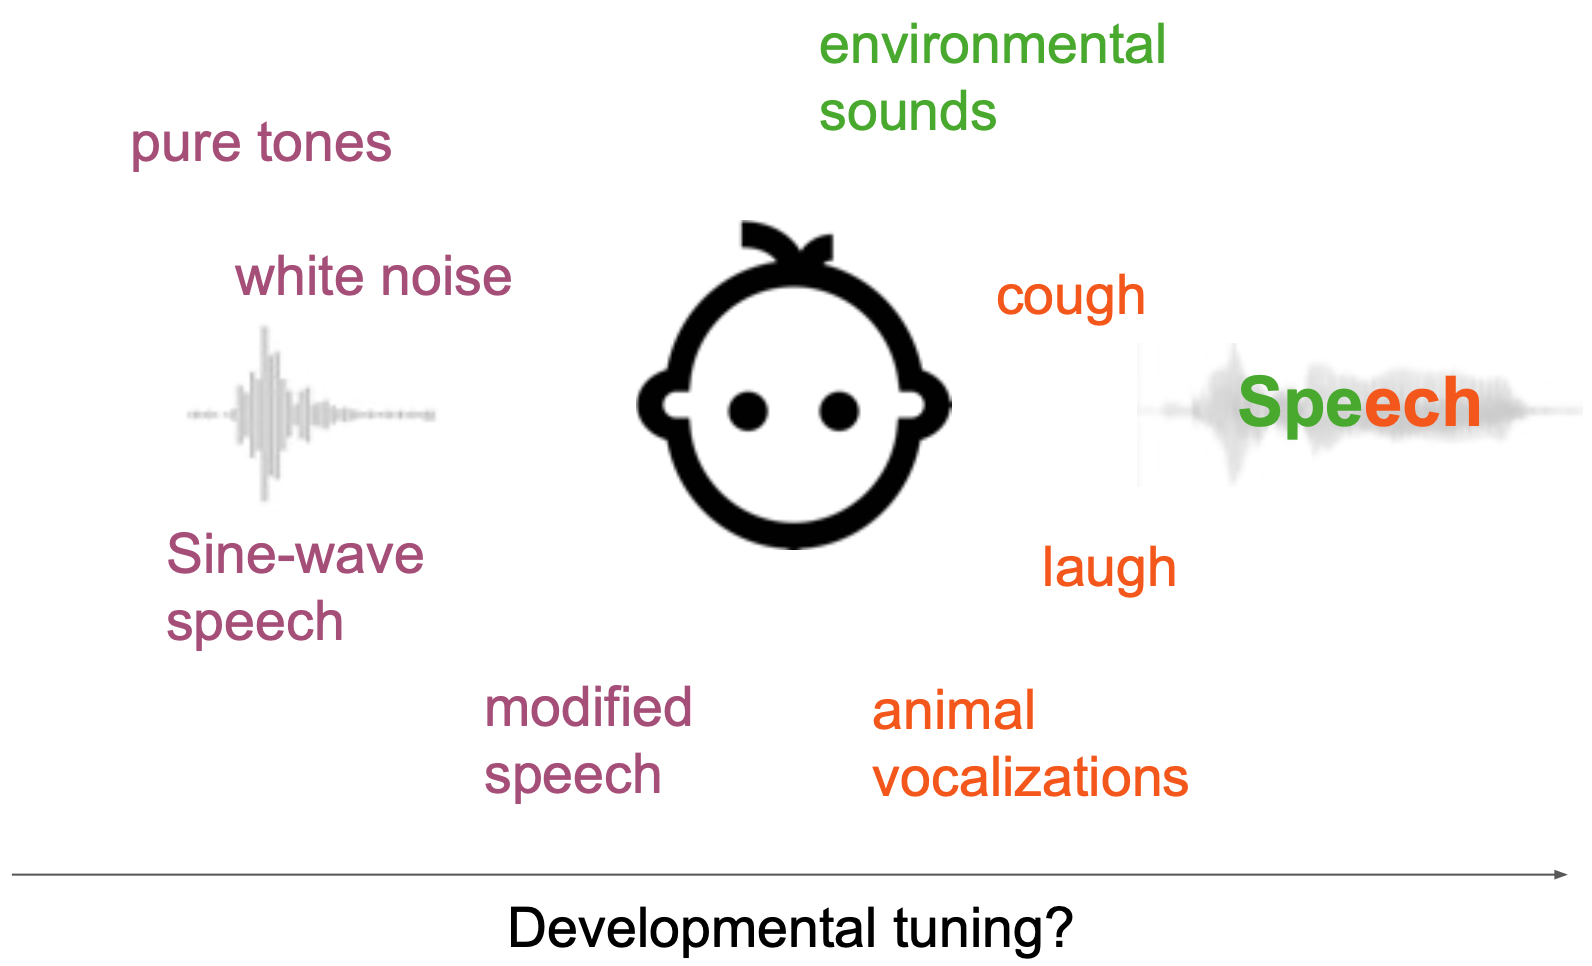
\includegraphics[width=5.31in]{figures_intro/tuning} \caption{Developmental tuning for speech in the first year of life: infant would first discriminate artificial (purple) and natural (green) sounds, then vocal sounds (orange) within natural sounds, and ultimately speech as a separate category within natural and vocal sounds.}\label{fig:tuning}
\end{figure}

\hypertarget{a-meta-analytic-approach}{%
\subsection{A meta-analytic approach}\label{a-meta-analytic-approach}}

Previous work has thus contributed both important hypotheses and tantalizing results, but the specificity of data collected in any one experiment makes it hard to obtain a bird's eye view. Moreover, some claims are based on juxtaposing a significant result in one condition or age against a non-significant one in another, a practice that is now known to be inappropriate since ``the difference between `significant' and `not significant' is not itself statistically significant'' (Gelman \& Stern, 2006). In this paper, we seek to directly test the theoretical predictions presented in the summarized work, namely that the preference for speech may be attributed to a general preference for vocalizations, to a preference for natural sounds, or to familiar sounds. To do so, we employ a meta-analytic approach, which is recommended over narrative reviews (Cristia, Tsuji, \& Bergmann, 2021). A meta-analysis can integrate data from experiments that vary in their methodology, as well as test the effect of factors of theoretical importance, by redescribing the stimuli used as a function of those factors. For instance, a study measuring preference for native speech over white noise provides data on a natural versus artificial contrast, as well as a vocal versus non-vocal contrast, thus accounting for how the same stimuli can be both natural and vocal or artificial and non-vocal.

Also, we can draw a developmental timeline across the age range covered by the literature, beyond age groups tested within papers. This is particularly useful in developmental psychology, which relies on age-related differences that need to be tested statistically (Gelman \& Stern, 2006). Meta-analyses offer a powerful statistical approach to directly test for interactions with age across the whole age-range covered by the literature. To give an example from a previous developmental meta-analysis, it had been proposed that infants' preference for novel or familiar items related to infants' age such that, all things equal, younger infants showed familiarity preferences whereas older infants exhibited novelty preferences (Hunter \& Ames, 1988). However, stable familiarity preferences across the first two years have been found for word segmentation in natural speech (Bergmann \& Cristia, 2016); and a stable novelty effect ensues for artificial grammars implemented in synthesized speech, whereas those implemented in natural speech led to stable familiarity preferences (Black \& Bergmann, 2017). Meta-analyses are therefore important to statistically and systematically test the theoretical predictions proposed in qualitative reviews, and show subtle effects that are difficult to see when reading the literature with a human eye.

Single experiments tell us about what a specific group of participants, presented with a specific set of stimuli, at a specific point in time has done. Meta-analyses are the following step because they provide a principled statistical approach to integrate those individual and specific results into a larger picture. By aggregating the numerous individual studies of a literature, meta-analyses gain statistical power. As a result, meta-analyses can reveal small effects that are difficult to show in individual experiments. By integrating data across different laboratories, they provide evidence for the generalizability of effects, and facilitate comparisons between experimental results. A systematic review also allows us to identify empirical gaps (e.g., age groups that are under-represented but are crucial to tease apart two factors) and conceptual gaps (e.g., use of stimuli that systematically confounds two or more of those explanations). As a result, meta-analyses are a moment of self-reflection for the field (Cox, Keren-Portnoy, Roepstorff, \& Fusaroli, 2022; Nguyen, Versyp, Cox, \& Fusaroli, 2021).

Finally, meta-analyses offer tools to detect publication bias in the literature. By aggregating all the available evidence for a phenomenon, we can see if the distribution of effect sizes has an unexpected shape, typically with an excess of positive results due to the difficulty to publish null or negative results. We can further integrate this information, and derive a new estimate of the overall effect size.

\hypertarget{research-question-and-predictions}{%
\subsection{Research question and predictions}\label{research-question-and-predictions}}

When an experiment uses native speech as the target and pure tones as the foil, the preference emerging could be due to at least four conceptually separable differences across the two stimuli types: One of them is speech and the other isn't, the former is produced with a mouth (vocal), it is a natural sound, and it is potentially more familiar than the latter. Can preferences observed in the previous body of work be explained by one of these factors?

If infants' (including newborns') preference is attributable to the fact that speech is a \textbf{vocal} sound, then effects when the competitor is vocal will be smaller than when it is not vocal. If it is driven by \textbf{naturalness}, then effects when the competitor is natural will be smaller than when it is not natural. Finally, if preferences are at least partly due to \textbf{familiarity}, then two predictions follow: effects should be larger when the target is the infant's native speech as opposed to foreign speech, and speech preference should increase with age. Of course, it is also possible that the preference for speech cannot be reduced to any of these three factors, in which case effect sizes will not be modulated by such distinctions. In addition, given that many previous empirical studies comment on changes with infant age, we pay special attention to the possibility that age modulates effect size in general, or specifically in conjunction with one of the aforementioned factors.

\hypertarget{methods}{%
\section{Methods}\label{methods}}

This meta-analysis was carried out following PRISMA recommendations (Moher, Liberati, Tetzlaff, Altman, \& Group, 2009). In addition, we provide information on all steps (including PRISMA checklist, data, and code) for full transparency and accountability via online supplementary materials; \url{https://osf.io/4stz9/?view_only=d0696591ebf34bfc8430f848cd945ca8}.

\hypertarget{literature-search}{%
\subsection{Literature search}\label{literature-search}}

We composed the initial list of papers with suggestions by experts (authors of this work); one google scholar search (\emph{(``speech preference'' OR ``own-species vocalization'') AND infant - ``infant-directed''}), the same search in PubMed and PsycInfo (last searched on 2019-09-24); and a google alert. We also inspected the reference lists of all included papers. Finally, we emailed a major mailing list to ask for missing data. We received two replies, one of which revealed a formerly undiscovered published study, and communicated unpublished data (Santolin, Zettersten, \& Saffran, 2020).

\hypertarget{inclusion-criteria}{%
\subsection{Inclusion criteria}\label{inclusion-criteria}}

As standard in systematic reviews, after a first screening based on titles and abstracts, we decided on final inclusion based on full paper reading. We included experiments that tested human infants from birth to one year of age, and contrasted speech sounds with any other type of sound, measuring behavioral preferences to the sounds (e.g., looking times). If a paper reported results from neurotypical and at-risk infants, we included only the data from the neurotypical group.

Given our key interest in the preference for speech over other sounds, we excluded studies that contrasted two different speech sounds (e.g., foreign vs.~native language, or adult vs.~child-directed speech, or mother vs.~stranger's voice); or two different non-speech sounds (e.g., backward speech vs.~animal vocalizations). In addition, we excluded experiments where the contrast presented to the infants could not be coded according to our three hypotheses (vocal, natural, familiar). This meant the exclusion of experiments where speech was presented in the mother's voice (which confounds speech and individual voice recognition for our familiarity factor). Finally, we excluded neuroimaging experiments to avoid mixing results from different brain regions with different response profiles. We included published (i.e., journal articles) as well as unpublished works (i.e., doctoral dissertations) as long as sufficient information was provided.

A PRISMA flow chart summarizes the literature review and selection process (Figure \ref{fig:prisma}). The full list of the papers that were inspected together with final inclusion decisions are available in a decision spreadsheet (see the online supplementary materials; \url{https://osf.io/4stz9/?view_only=d0696591ebf34bfc8430f848cd945ca8}).

\begin{figure}
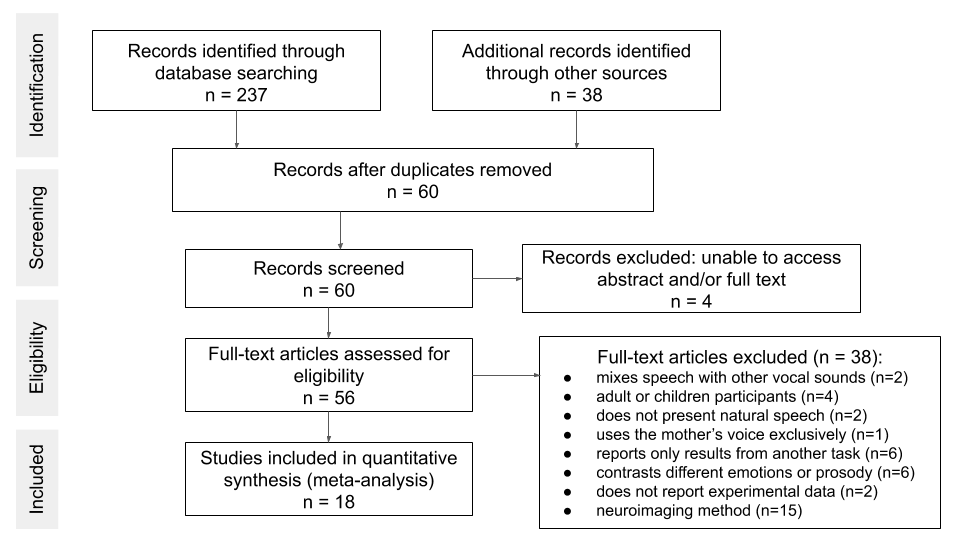
\includegraphics[width=3.2in]{figures_intro/PRISMA} \caption{PRISMA flowchart summarizing the literature review and selection process.}\label{fig:prisma}
\end{figure}

\hypertarget{coding}{%
\subsection{Coding}\label{coding}}

Data were coded by the first author. In addition, 20\% of the papers were randomly selected to be coded by the last author independently, with disagreements resolved by discussion. There were 10 disagreements out of a total of 260 fields filled in, and they were indicative of the coders not following the codebook, which led to a revision of all data in four variables.

The critical variables for our purpose are key stimuli characteristics, infant age, and testing method (central fixation, high amplitude sucking, head-turn preference procedure). As for key stimuli characteristics, we coded vocal quality, naturalness, and familiarity, as follows.

For \textbf{vocal quality}, the competitor sound was considered as vocal if it was produced by an animal vocal tract (human or not), either original or modified. Vocal competitors included non-speech vocalizations, animal calls, bird song, and filtered speech. Non-vocal competitors included backward speech (that has abrupt closures that cannot be produced by a vocal tract), white-noise, environmental sounds, instrumental music, heartbeat, and sine-wave speech (that lacks the harmonic structure introduced by the natural resonance of the vocal tract).

For \textbf{naturalness}, the competitor sound was coded as natural if it was produced by a biological organism without any further acoustic manipulation. Natural competitors included animal calls, environmental sounds (e.g.~wind or water sounds), heartbeat, bird song, non-speech vocalizations (e.g.~laughter or coughs). If the authors applied acoustic manipulations, the competitor was coded as artificial. Artificial competitors included sine-wave speech, filtered speech\footnote{In the case of filtered speech, the modulations introduced by the vocal tract are still present at the retained frequencies, and formant transitions are consistent with vocal production constraints. For this reason, filtered speech can be considered as vocal but not natural.
  For \textbf{familiarity}, we considered the language in which the speech sounds were recorded (native or foreign).}, white noise, instrumental music, and speech with altered rhythmic structure. The only exception was for newborn experiments presenting low-pass filtered speech mimicking the filtering applied by the womb. Given the recency of the intra-uterine environment to newborns (about 2 days), we coded these as natural.

We coded all the statistical information reported in the included papers. If reported, we coded the mean score and the standard deviation for speech, and the other sound separately. When infant-level data was provided, we recomputed the respective mean scores and standard deviations based on the reported individual scores. If reported, we also coded the t-statistic between the two sound conditions, or an F-statistic provided this was a two-way comparison. If effect sizes were directly reported as a Cohen's d or a Hedges' g, we also coded this.

\hypertarget{effect-sizes}{%
\subsection{Effect sizes}\label{effect-sizes}}

Once the data were coded, we extracted effect sizes, along with their respective variance. Effect sizes were standardized differences (Cohen's d) between response to speech vs.~the competitor.
If effect sizes were not directly reported in the papers, we computed them using the respective means and SDs (Lipsey \& Wilson, 2001), or a t- or F-statistic (Dunlap, Cortina, Vaslow, \& Burke, 1996). As our effect sizes came from within-subject comparisons (e.g., looking time of the same infant during speech and monkey calls), we needed to take into account the correlation between the two measurements in effect sizes and effect size variances computations. We computed this correlation based on the t-statistic, the respective means, and SDs (Lipsey \& Wilson, 2001) if they were all reported; or imputed this correlation randomly if not (Bergmann \& Cristia, 2016). We calculated the variance of each effect size using standard formulae (Lipsey \& Wilson, 2001). Cohen's d were transformed to Hedges' g by multiplying d by a correction factor for small sample sizes based on the degrees of freedom (Borenstein, Hedges, Higgins, \& Rothstein, 2011).

We did not center age because our hypotheses included a developmental progression from birth to the end of the first year of life. We were therefore interested in the intercept at age 0 (i.e., birth).

Analyses use the R (R Core Team, 2018) package Robumeta (Hedges, Tipton, \& Johnson, 2010), which allows us to fit meta-analytic regressions that take into account the correlated structure of the data when repeated measures are obtained from the same infant groups within papers (Bergmann et al., 2018).

\hypertarget{results}{%
\section{Results}\label{results}}

\hypertarget{database-description}{%
\subsection{Database description}\label{database-description}}

We found a total of 19 publications (labeled with an asterisk in the reference list) reporting 39 experiments, for a total of 791 infants, and 55 (not mutually independent) effect sizes. Regarding publication status, 47 effect sizes came from 16 papers that have been \textbf{submitted to or} published in peer-reviewed journals (Colombo \& Bundy, 1981; Cooper \& Aslin, 1994; Curtin \& Vouloumanos, 2013; Ecklund-Flores \& Turkewitz, 1996; Santolin, Russo, Calignano, Saffran, \& Valenza, 2019; Segal \& Kishon-Rabin, 2011; Segal, Kligler, \& Kishon-Rabin, 2021; Shultz \& Vouloumanos, 2010; Sorcinelli, Ference, Curtin, \& Vouloumanos, 2019; Spence \& DeCasper, 1987; Vanden Bosch der Nederlanden \& Vouloumanos, 2021; Vouloumanos \& Curtin, 2014; Vouloumanos, Druhen, Hauser, \& Huizink, 2009; Vouloumanos et al., 2010, 2010; Vouloumanos \& Werker, 2004; Vouloumanos \& Werker, 2007; Yamashiro, Curtin, \& Vouloumanos, 2020). Additionally, a thesis contributed 5 effect sizes (Ference, 2018), and 3 effect sizes were contributed by authors of unpublished work (Santolin et al., 2020).

Experiments tended to have small sample sizes, with a median N of 16 children (Range = {[}4, 60{]}, M = 19.76), which is close to the field standard (Bergmann et al., 2018), but much lower than current recommendations (Oakes, 2017). Infants ranged from 0 to 12 months (1.50 to 380.50 days), although the majority were under 6 months of age (61.54\% of the experiments).

There was a fair representation of the factors most relevant to the theoretical hypotheses we aimed to assess. Speech stimuli were recorded in the infant native language in 64.10\% of the experiments.
The competitor sound was vocal in 46.15\% of the experiments. The competitor sound was natural 46.15\% of the experiments. Although this means there is some data to assess each of the hypotheses, our systematic review also reveals that these factors are not very well separated in previous work. To start with the most obvious case in which two theoretical explanations are hard to tease apart, there was only 15.38\% of effects emerging from stimuli that were natural but not vocal, 10.26\% that we classified as vocal but not natural (filtered speech), 46.15\% that were neither natural nor vocal, and the rest that were both natural and vocal (35.90\%). This means that if we find that both naturalness and vocalness explain effect sizes, we cannot properly attribute variance to one or the other.

Less obvious is the fact that there are confounds across vocal, natural, and familiarity factors. Figure \ref{fig:stimuli} shows that there are relatively fewer effect sizes in which foreign speech is contrasted against non-vocal sounds, and against non-natural sounds, for which we have less than 10 (non-independent) effect sizes. Again, this means that it will be difficult to attribute unique variance to familiarity versus the other factors, if they emerge as significant predictors. In addition, we note that experiments using the infants' native language tested infants from the whole range covered in this meta-analysis (0 to 12 months of age), whereas experiments using a foreign language only tested infants from 3 to 9 months of age, a point to which return.

\begin{figure}
\centering
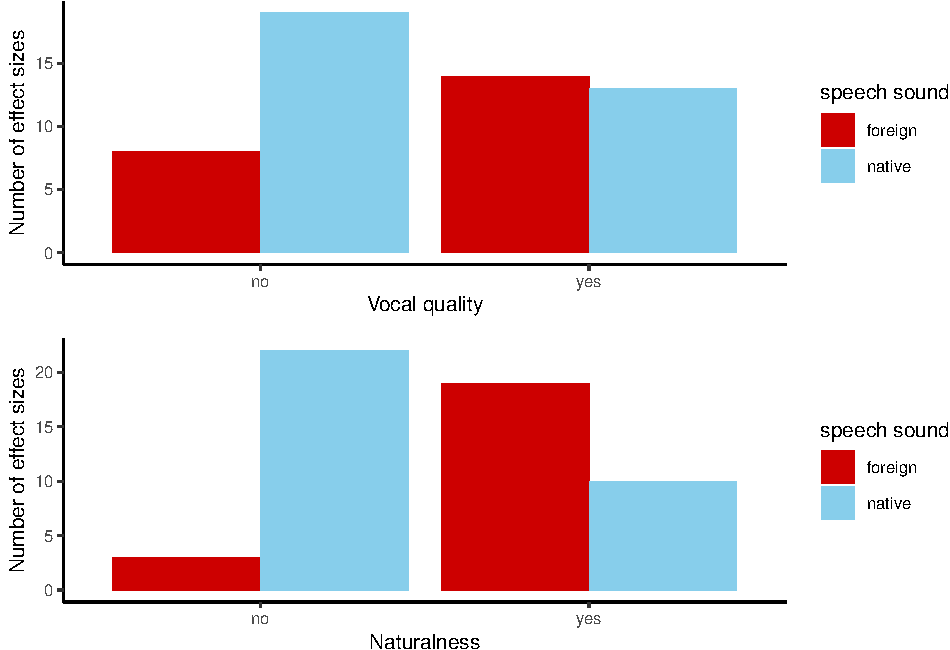
\includegraphics{MA_speech_pref_files/figure-latex/stimuli-1.pdf}
\caption{\label{fig:stimuli}Histograms of the number of effect sizes for each language and moderator status.}
\end{figure}

Although not integral to our study, we report characteristics of discovered data along other dimensions, which are relevant when considering the likely generalizability of conclusions based on previous empirical work. Individual samples comprised 46\% of female participants on average. Infants were native of 6 different languages across the whole database (English, French, Russian, Yiddish, Hebrew, Italian).
Experiments were performed in 10 different laboratories from 4 different countries (United States, Canada, Israel, Italy). 3 experimental methods were used: 79.49\% of the experiments used Central Fixation (CF, also called sequential looking preference procedure); 7.69\% used High-Amplitude Sucking (HAS); and 12.82\% used Head-turn Preference Procedure (HPP). Trial length was fixed in 20.51\% of the experiments, and infant-controlled in 76.92\% of the experiments.

Speech sounds were spoken by a female in 94.87\% of the experiments, with an infant-directed prosody in 53.85\% of the experiments. Speech was presented in isolated segments (i.e.~words or syllables) in 10.26\% of the experiments, and full sentences or passages in 48.72\% of the experiments (the remaining were unspecified). The competitors covered a wide range of sounds, as represented in Figure \ref{fig:competitors}.\footnote{A consistent body of literature suggests that infants prefer infant-directed over adult-directed speech (ManyBabies Consortium, 2020). Although these studies assessed the preference between two different speech sounds, and not speech and another type of sound, one could argue that this phenomenon could drive the preference for speech over another type of sound. To control for this confound, we ran a model with age and prosody (ADS/IDS) as factors. We found no effect of either of these factors (Supplementary results S3, Supplementary Figure S4).
}

\begin{figure}
\centering
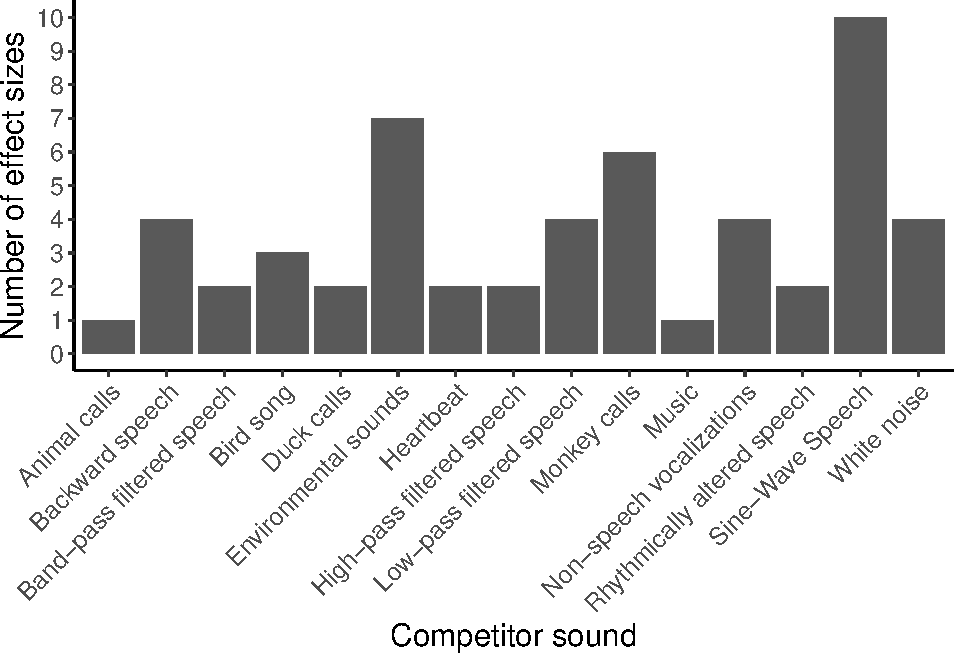
\includegraphics{MA_speech_pref_files/figure-latex/competitors-1.pdf}
\caption{\label{fig:competitors}Histogram of the number of effect sizes for each competitor.}
\end{figure}

\hypertarget{average-effect-size}{%
\subsection{Average effect size}\label{average-effect-size}}

\begin{figure}
\centering
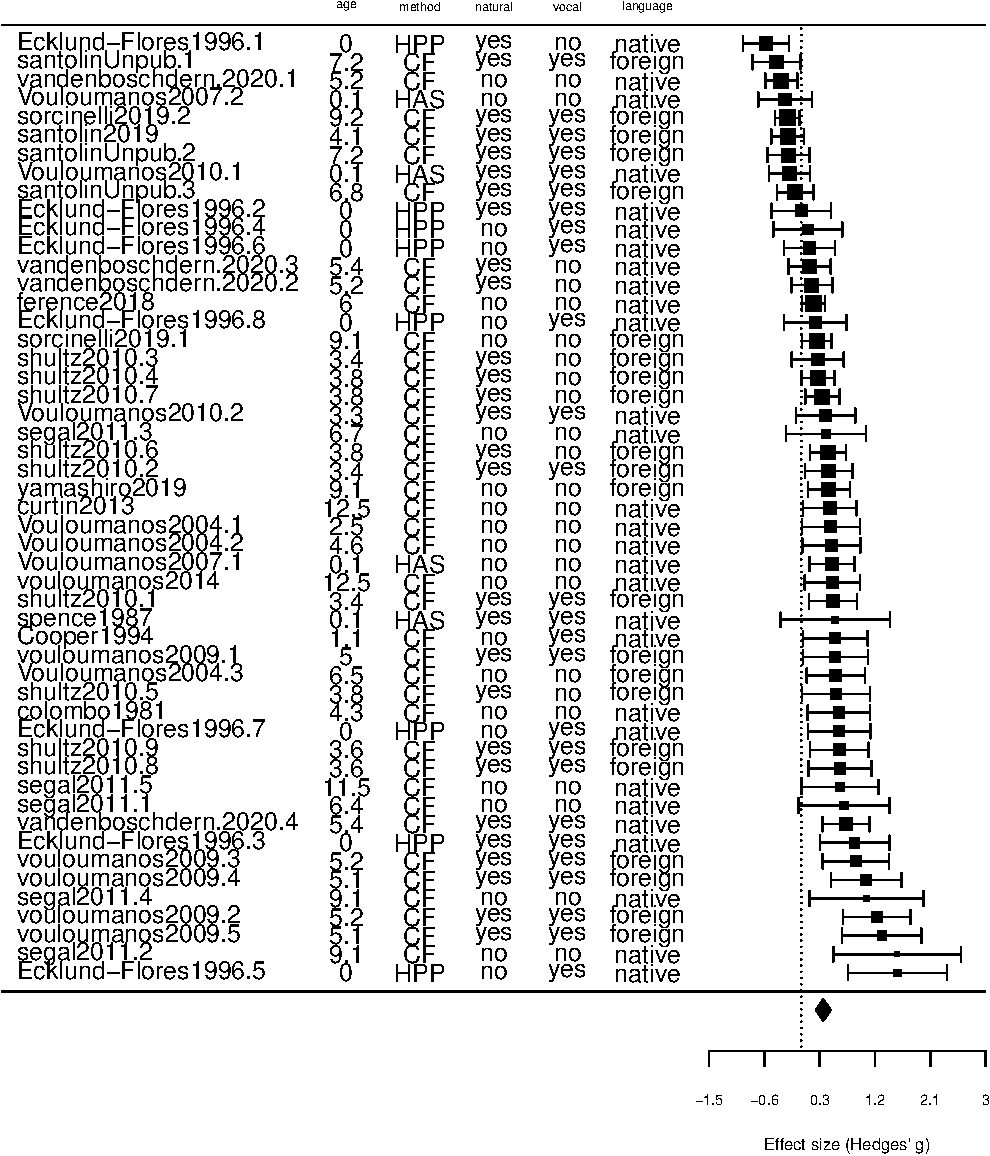
\includegraphics{MA_speech_pref_files/figure-latex/forest-1.pdf}
\caption{\label{fig:forest}Forest plot of effect sizes available in the literature, along with their respective moderator status. The average effect size is plotted on the bottom line.}
\end{figure}

Following standard analytic practice, we removed 3 outliers that were more than 3 standard deviations away from the mean. We then integrated all effect sizes in a meta-analytic regression without any moderator, and found an average effect size g of 0.40 (SE = 0.07, CI = {[}0.26 , 0.55{]}) (see Figure \ref{fig:forest} for the forest plot), corresponding to a medium effect size for the literature as a whole, which was significantly different from zero (\(t\) = 5.59, \(p\) \textless{} .001).
Heterogeneity among effect sizes was estimated at \(\tau^2\) = 0.16 (I\textsuperscript{2} = 78.38\%), which was significant (Q = 206.59, p \textless{} 0.01) despite the removal of outliers before running the model. This strongly suggest differences across experiments, and invites analyses using moderators.

\hypertarget{publication-bias}{%
\subsection{Publication bias}\label{publication-bias}}

\begin{figure}
\centering
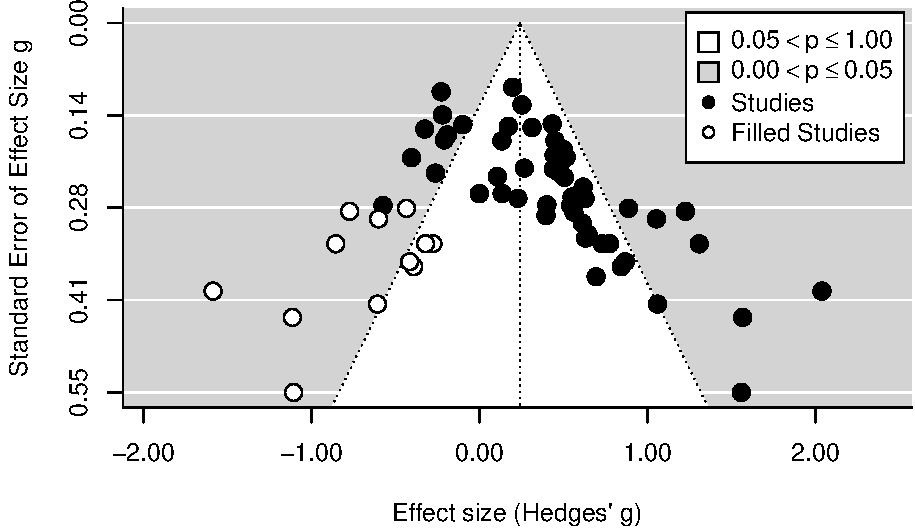
\includegraphics{MA_speech_pref_files/figure-latex/bias-1.pdf}
\caption{\label{fig:bias}Funnel plot of effect sizes and their respective standard errors. Black dots: effect sizes observed in the literature. White dots: missing effect sizes, suggestive of a publication bias\(^2\). Vertical line: average effect size after filling the missing effect sizes.}
\end{figure}

Before proceeding with the moderator analysis, we checked for the presence of a potential publication bias in the body of literature by studying the relationship between standard errors of effect sizes as a function of Hedges' g (see funnel plot in Figure \ref{fig:bias})\footnote{If the literature is not biased, effect sizes should be evenly distributed around the mean effect size, with increasing standard error as they go away from the mean effect size (both in the positive and negative directions, white triangle in the funnel plot). This is reflected by a symmetrical funnel plot, with no linear relationship between effect sizes and standard errors.}. A regression test on these data was significant (z = 6.70, p \textless{} 0.01), as was the Kendall's tau rank correlation test for funnel plot asymmetry (Kendall's tau = 0.52, p \textless{} 0.01), consistent with a publication bias in the literature.

To check whether this bias fully explains speech preference in the extant body of literature, we symmetrized the funnel plot with the ``trim and fill'' method (Duval \& Tweedie, 2000). To symmetrize the funnel plot, 12 (SE = 4.75) missing experiments were needed on the left side of the plot. The corrected effect size was estimated at 0.24 (SE = 0.07) after filling in the 12 missing experiments, which is still significantly different from zero. Thus, even correcting for a potential publication bias, we still find statistical evidence for infants' preferring speech over competitors.

\hypertarget{moderator-analyses}{%
\subsection{Moderator analyses}\label{moderator-analyses}}

We then tested if heterogeneity could be accounted for by the factors proposed in previous work (vocal, natural, familiar). There are two main ways of answering this question, and they provide converging results. We start with the simplest analysis, in which a single meta-analytic model is fit with the following moderators:

\begin{itemize}
\tightlist
\item
  mean age of children;
\item
  vocal quality of the competitor sound (coded as yes if it was vocal and no otherwise);
\item
  naturalness of the competitor sound (coded as yes if it was natural and no otherwise);
\item
  familiarity with the language used (native or foreign).
\end{itemize}

These moderators were specified without interactions with each other both to avoid overfitting and because they were sometimes confounded in previous work, as described previously. None of the moderators was significant in this analysis (see Table \ref{tab:Table2}).

\begin{table}[tbp]

\begin{center}
\begin{threeparttable}

\caption{\label{tab:Table2}Statistical results of meta-regression with all moderators. The intercept corresponds to the effect size when the competitor is natural, and vocal, and speech is in a foreign language, at age 0. The moderator estimates correspond to changes in the intercept when the target stimuli are in the native language (familiarity); the competitor is artificial (naturalness); and the competitor is non-vocal (vocal quality).}

\begin{tabular}{lcccc}
\toprule
 & estimate & SE & t & confidence interval\\
\midrule
intercept & 0.17 & 0.17 & 0.98 & -0.19 - 0.54\\
naturalness & 0.00 & 0.00 & 0.87 & 0 - 0\\
vocal quality & -0.09 & 0.16 & -0.55 & -0.45 - 0.27\\
language & 0.27 & 0.13 & 2.02 & -0.02 - 0.55\\
age & 0.05 & 0.16 & 0.34 & -0.28 - 0.39\\
\bottomrule
\end{tabular}

\end{threeparttable}
\end{center}

\end{table}

\begin{figure}
\centering
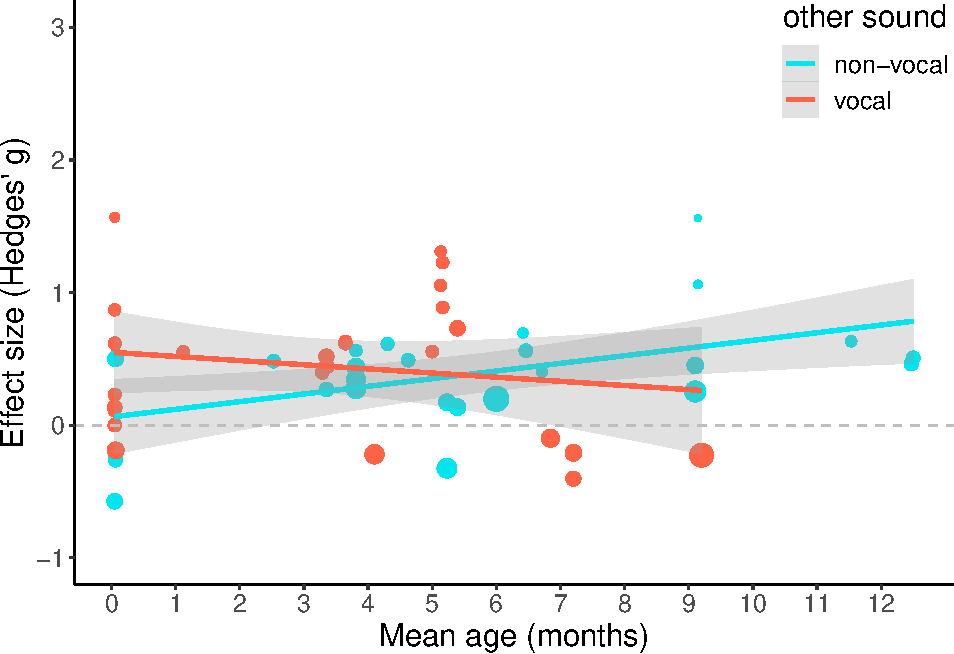
\includegraphics{MA_speech_pref_files/figure-latex/vocal-1.pdf}
\caption{\label{fig:vocal}Effect sizes as a function of age and vocal quality of the competitor. The size of each dot is inversely proportional to the variance. Positive effect sizes reflect a preference for the speech sound, negative effect sizes reflect a preference for the competitor sound.}
\end{figure}

\begin{table}[tbp]

\begin{center}
\begin{threeparttable}

\caption{\label{tab:TableVocal}Statistical results of meta-regression with vocal quality and its interaction with age as moderators. The intercept corresponds to the effect size when the competitor is vocal, at age 0. The moderator estimates correspond to changes in the intercept when the competitor is non-vocal (vocal quality).}

\begin{tabular}{lcccc}
\toprule
 & estimate & SE & t & confidence interval\\
\midrule
intercept & 0.48 & 0.15 & 3.17 & 0.13 - 0.83\\
vocal quality & -0.40 & 0.22 & -1.86 & -0.86 - 0.06\\
vocal quality*age & 0.00 & 0.00 & 2.40 & 0 - 0.01\\
\bottomrule
\end{tabular}

\end{threeparttable}
\end{center}

\end{table}

\begin{figure}
\centering
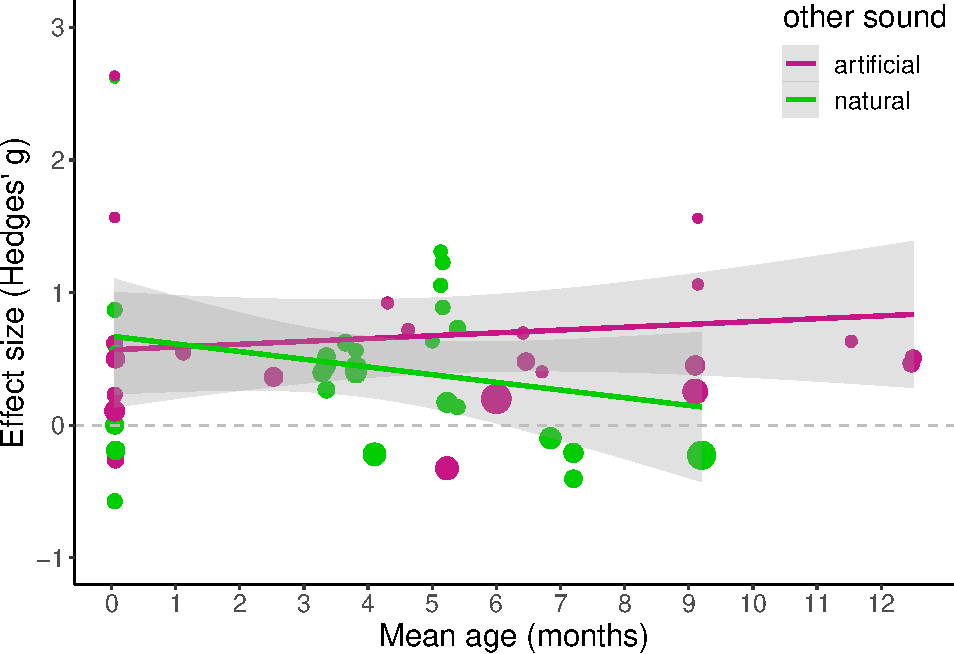
\includegraphics{MA_speech_pref_files/figure-latex/natural-1.pdf}
\caption{\label{fig:natural}Effect sizes as a function of age and natural quality of the competitor. The size of each dot is inversely proportional to the variance. Positive effect sizes reflect a preference for the speech sound, negative effect sizes reflect a preference for the competitor sound.}
\end{figure}

\begin{table}[tbp]

\begin{center}
\begin{threeparttable}

\caption{\label{tab:TableNatural}Statistical results of meta-regression with naturalness and its interaction with age as moderators. The intercept corresponds to the effect size when the competitor is natural, at age 0. The moderator estimates correspond to changes in the intercept when the competitor is artificial (naturalness).}

\begin{tabular}{lcccc}
\toprule
 & estimate & SE & t & confidence interval\\
\midrule
intercept & 0.36 & 0.21 & 1.67 & -0.17 - 0.88\\
naturalness & 0.00 & 0.24 & 0.00 & -0.53 - 0.52\\
naturalness*age & 0.00 & 0.00 & 1.05 & 0 - 0.01\\
\bottomrule
\end{tabular}

\end{threeparttable}
\end{center}

\end{table}

\begin{figure}
\centering
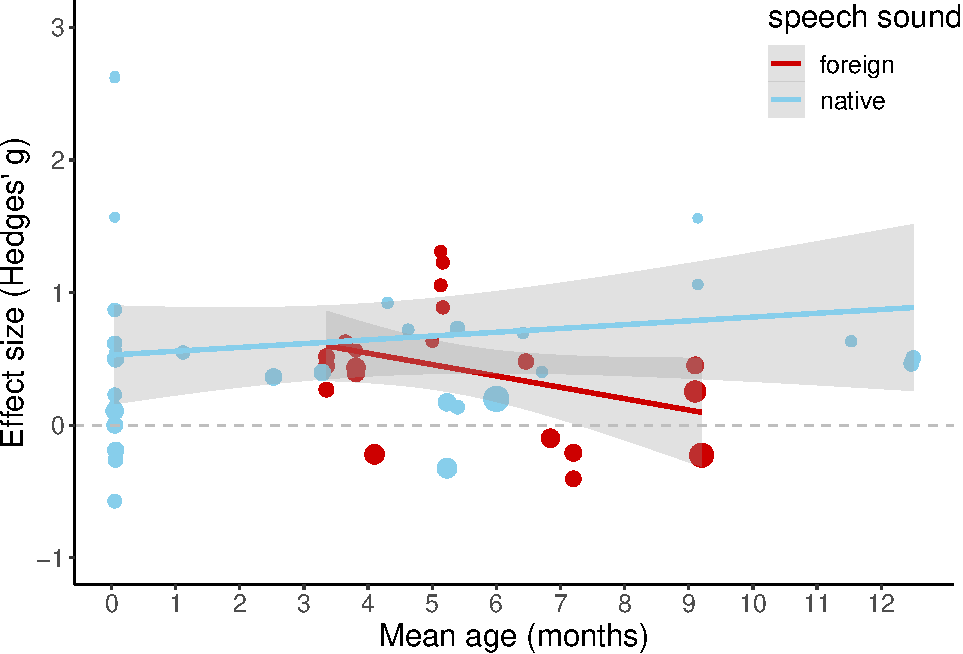
\includegraphics{MA_speech_pref_files/figure-latex/lang-1.pdf}
\caption{\label{fig:lang}Effect sizes as a function of age and familiarity with the speech sounds. The size of each dot is inversely proportional to the variance. Positive effect sizes reflect a preference for the speech sound, negative effect sizes reflect a preference for the competitor sound.}
\end{figure}

\begin{table}[tbp]

\begin{center}
\begin{threeparttable}

\caption{\label{tab:TableLang}Statistical results of meta-regression with language of the speech sounds and interaction with age. The intercept corresponds to the effect size when speech is in a foreign language at age 0. The moderator estimate correspond to changes in the intercept when the target stimuli are in the native language.}

\begin{tabular}{lcccc}
\toprule
 & estimate & SE & t & confidence interval\\
\midrule
intercept & 0.72 & 0.30 & 2.44 & 0.03 - 1.41\\
language & -0.48 & 0.32 & -1.52 & -1.19 - 0.22\\
language * age & 0.00 & 0.00 & 2.24 & 0 - 0.01\\
\bottomrule
\end{tabular}

\end{threeparttable}
\end{center}

\end{table}

Another way of answering our key research question is by fitting a separate meta-regression model for each moderator and its interaction with age. Once again, we observe no significant main effect (nor interaction with age) for a meta-regression declaring vocal quality of the competitor (Figure \ref{fig:vocal}, Table \ref{tab:TableVocal}), naturalness of the competitor (Figure \ref{fig:natural}, and Table) \ref{tab:TableNatural}), or whether the speech was foreign or native (Figure \ref{fig:lang}, and Table \ref{tab:TableLang}).

\hypertarget{discussion}{%
\section{Discussion}\label{discussion}}

Our meta-analysis synthesizes the available literature on infants' preference for speech sounds. When all experiments were considered together with no moderators, we found a sizable intercept (g=0.40, g=0.24 when taking the publication bias into account), which was still significant after correcting for the publication bias. Our meta-analysis shows that this preferential processing of speech sounds is observable from birth on. It is important to stress that this conclusion is not trivial because others have said similar things in the past: One key advantage of meta-analysis over conclusions drawn from individual studies or unsystematic narrative reviews is that we can actually measure the likely presence of publication bias (which \emph{is} present in these data, as we discuss below), and furthermore compensate for this bias statistically, to see if an effect remains significant after doing so (Cristia et al., 2021; see also Ioannidis, 2005).

The significant heterogeneity we found among the literature suggests that underlying factors modulate this effect. Based on previous theoretical claims, one would have predicted infants' speech preference to be larger when the competitor was non-vocal; when the competitor was an artificial sound than when it was a natural one; and when the speech was in the infants' native language. In fact, we were unable to disprove the null hypothesis of no difference for all three factors. Thus, although these explanations are conceptually appealing, it does not appear to be the case that we can reduce infants' speech preference to a bias for vocal, natural, or familiar sounds.

Also based on theoretical claims in the literature, we had expected age to play a major role. Indeed, experiments comparing the preference for human speech against human non-speech as well as animal vocalizations more generally (McDonald et al., 2019; Vouloumanos et al., 2010) often discuss age-related differences in categorization of these sounds. Surprisingly, age did not significantly moderate the overall preference for speech, as shown by the null estimate of this moderator (Table \ref{tab:Table2}), nor did it interact with any other moderators (Tables \ref{tab:TableNatural}, \ref{tab:TableLang}, and \ref{tab:TableVocal}, and corresponding figures). This result was replicated in a separate model declaring age as the only moderator, which showed a significant intercept, similar in size to the intercept found in the meta-regression with no moderator (Supplementary results S1).
Crucially, in this supplementary analysis, age was not centered so that this intercept provides an estimate of the effect size at age 0, i.e.~at birth.
Moreover, the scatterplot of effect sizes as a function of age reveals clearly no change with age even when plotted without other moderators (Supplementary figure S2). This null effect of age, combined with the sizable intercept, confirms that infants reliably prefer speech over other types of sounds stably across the age range covered by previous literature.

For all of our analyses, concerning vocal quality, naturalness, familiarity, and age, it is important to remember that, by aggregating the numerous individual studies of a literature, meta-analyses gain statistical power as compared to individual experiments. As such, meta-analytic results have more cumulative explanatory value than single studies.

Our meta-analysis revealed uneven distributions of experiments across age and stimulus dimensions, and that the distribution of effect sizes in the literature is consistent with publication bias. Moreover, distributions of effect sizes for experiments varying along the three dimensions widely overlap.

This clearly points to the value of meta-analysis: to take stock of a field and inspire follow-up studies. In particular, future experiments should test infants from 1 to 3 months, and older than 9 months. Language production gains in complexity at about 9 months (Oller, Eilers, Neal, \& Schwartz, 1999), which could affect infants' speech preference. Experiments using natural vocal stimuli as competitor, and foreign speech as target, would contribute to fill in the gap in the literature that our meta-analysis revealed. Our dataset can be community-augmented, and we invite researchers investigating this phenomenon to complement it with any data they would have (\url{https://osf.io/4stz9/?view_only=d0696591ebf34bfc8430f848cd945ca8}), whatever the results and publication status, to address the current publication bias currently affecting this body of work, and potentially revisit the research question that motivated the present study.

Our results suggest that, from birth on, infants show a preference for speech, which cannot be accounted by the three explanations tested here: vocal quality, naturalness, or familiarity with the native language. It is possible that infants prefer speech because of its complex acoustic structure and fast transitions (Rosen \& Iverson, 2007). Spectral or temporal modulations taken separately are not sufficient to elicit neural responses similar to the ones elicited by speech (Minagawa-Kawai, Cristià, Vendelin, Cabrol, \& Dupoux, 2011). However, speech is characterized by joint spectrotemporal modulations at specific rates (Singh \& Theunissen, 2003). It is possible that infants are sensitive to this specific spectro-temporal structure (though see Norman-Haignere \& McDermott, 2018 showing that they only explain neural responses in primary auditory cortex, suggesting that other factors contribute to the behavioral response in later processing stages). Testing this explanation would require to compute the modulation spectra of the actual stimuli used in the experiments. Thus, we recommend interested researchers to deposit their stimuli in a public archive such as the Open Science Framework (Foster \& Deardorff, 2017).

A stable preference for speech in infancy is compatible with the idea that infants are born with the capacity to recognize their conspecifics' communication signals. This parallels what has been proposed for faces: Infants are born with the capacity to orient their attention toward them, even without any prior exposure to faces (Morton \& Johnson, 1991; Turati, 2004).
This would stem from basic perceptual abilities present at birth, namely that the visual system would be tuned to a spatial structure that correspond to those of faces (Morton \& Johnson, 1991; Turati, 2004). As newborns have never been exposed to such visual stimuli before, it would reflect general properties (i.e.~filters) of the visual system. Similarly, the auditory system could be tuned to a spectro-temporal structure that speech presents. The combination of this non-specific bias with the systematic variations of the auditory environment (i.e.~the fact that an acoustical structure characterizes speech but not other sounds of the environment) would result in preferential responses to speech from birth. However, contrary to faces, fetuses are exposed to speech low-pass filtered by the womb throughout the last trimester of gestation (Lecanuet \& Granier-Deferre, 1993; Querleu, Renard, Versyp, Paris-Delrue, \& Crèpin, 1988). It is therefore possible that prenatal experience with low-pass filtered speech helps infants to form a representation of speech, by tuning the response properties of the auditory system to speech.
The fact that familiarity with the language used in the experiment did not modulate infants' preference suggests that this effect is not triggered by familiarity with the sounds of the native language. Infants would therefore form a representation that is specific enough to discriminate speech from other natural or vocal sounds, but general enough to be independent of the language spoken.

The human species is a gregarious one. Detecting speech signals allows to integrate it with other sensory percepts, such as faces, to form multisensory representations of conspecifics. Five-months old infants were capable to match human faces to speech, as well as monkey faces to monkey vocalizations (Vouloumanos et al., 2009). This provides evidence that human infants make correspondences between faces and vocalizations, and that they distinguish their conspecifics from other species. This lays the groundwork for social cognition. Finally, the preference itself may also be a meaningful index of processing that can be used to identify children at risk (Sorcinelli et al., 2019). Understanding this phenomenon is therefore crucial for both theoretical and clinical advances.

Ultimately, preferential processing of speech may support higher level cognitive tasks. Identifying speech signals and paying attention to them would allow infants to form complex representations of the sensory world, that they can manipulate cognitively. Consistently, infants could categorize visual stimuli (i.e., associate a label to a category of objects) when they were associated to speech, but not pure tones or backward speech (Ferry, Hespos, \& Waxman, 2010, 2013; Fulkerson \& Waxman, 2007). Interestingly, infants categorized visual stimuli when presented with speech, melodies, monkey (Fulkerson \& Haaf, 2003), or lemur vocalizations (Ferry et al., 2013). These results support the idea that infants' cognition is set up to respond to, and manipulate complex sounds (i.e.~modulated in time and frequency), especially those of critical ecological importance such as communicative vocalizations.

With a sample size of 791 infants, covering the wide age range of all individual experiments available, our meta-analysis provides evidence for a specialized processing of speech from birth. This parallels infants' attention to faces from birth (Morton \& Johnson, 1991; Turati, 2004), and suggests that human cognition is set up to pay attention to signals from conspecifics specifically. Such systems may be the precursors of humans' advanced social cognition skills.

\newpage

\hypertarget{references}{%
\section{References}\label{references}}

\begingroup
\setlength{\parindent}{-0.5in}
\setlength{\leftskip}{0.5in}

References marked with an asterisk indicate studies included in the meta-analysis.

\hypertarget{refs}{}
\begin{CSLReferences}{1}{0}
\leavevmode\vadjust pre{\hypertarget{ref-bergmann_development_2016}{}}%
Bergmann, C., \& Cristia, A. (2016). Development of infants' segmentation of words from native speech: A meta-analytic approach. \emph{Developmental Science}, \emph{19}(6), 901--917. \url{https://doi.org/10.1111/desc.12341}

\leavevmode\vadjust pre{\hypertarget{ref-bergmann_promoting_2018}{}}%
Bergmann, C., Tsuji, S., Piccinini, P. E., Lewis, M. L., Braginsky, M., Frank, M. C., \& Cristia, A. (2018). Promoting {Replicability} in {Developmental} {Research} {Through} {Meta}-analyses: {Insights} {From} {Language} {Acquisition} {Research}. \emph{Child Development}, \emph{89}(6), 1996--2009. \url{https://doi.org/10.1111/cdev.13079}

\leavevmode\vadjust pre{\hypertarget{ref-bertoncini_morae_1995}{}}%
Bertoncini, J., Floccia, C., Nazzi, T., \& Mehler, J. (1995). Morae and {Syllables}: {Rhythmical} {Basis} of {Speech} {Representations} in {Neonates}. \emph{Language and Speech}, \emph{38}(4), 311--329. \url{https://doi.org/10.1177/002383099503800401}

\leavevmode\vadjust pre{\hypertarget{ref-black_quantifying_2017}{}}%
Black, A., \& Bergmann, C. (2017). \emph{Quantifying infants' statistical word segmentation: {A} meta-analysis}. 124--129. Cognitive Science Society. Retrieved from \url{https://pure.mpg.de/pubman/faces/ViewItemOverviewPage.jsp?itemId=item_2475527}

\leavevmode\vadjust pre{\hypertarget{ref-borenstein_introduction_2011}{}}%
Borenstein, M., Hedges, L. V., Higgins, J. P. T., \& Rothstein, H. R. (2011). \emph{Introduction to {Meta}-{Analysis}}. John Wiley \& Sons.

\leavevmode\vadjust pre{\hypertarget{ref-colombo_method_1981}{}}%
Colombo, J., \& Bundy, R. S. (1981). A method for the measurement of infant auditory selectivity. \emph{Infant Behavior and Development}, \emph{4}, 219--223. \url{https://doi.org/10.1016/S0163-6383(81)80025-2}

\leavevmode\vadjust pre{\hypertarget{ref-cooper_developmental_1994}{}}%
Cooper, R. P., \& Aslin, R. N. (1994). Developmental {Differences} in {Infant} {Attention} to the {Spectral} {Properties} of {Infant}-{Directed} {Speech}. \emph{Child Development}, \emph{65}(6), 1663--1677. \url{https://doi.org/10.2307/1131286}

\leavevmode\vadjust pre{\hypertarget{ref-cox2022bayesian}{}}%
Cox, C. M. M., Keren-Portnoy, T., Roepstorff, A., \& Fusaroli, R. (2022). A bayesian meta-analysis of infants? Ability to perceive audio--visual congruence for speech. \emph{Infancy}, \emph{27}(1), 67--96.

\leavevmode\vadjust pre{\hypertarget{ref-cristia_meta-analytic_2021}{}}%
Cristia, A., Tsuji, S., \& Bergmann, C. (2021). A meta-analytic approach to evaluating the explanatory adequacy of theories. In \emph{MetaPsychology}. OSF Preprints. \url{https://doi.org/10.31219/osf.io/83kg2}

\leavevmode\vadjust pre{\hypertarget{ref-curtin_speech_2013}{}}%
Curtin, S., \& Vouloumanos, A. (2013). Speech {Preference} is {Associated} with {Autistic}-{Like} {Behavior} in 18-{Months}-{Olds} at {Risk} for {Autism} {Spectrum} {Disorder}. \emph{Journal of Autism and Developmental Disorders}, \emph{43}(9), 2114--2120. \url{https://doi.org/10.1007/s10803-013-1759-1}

\leavevmode\vadjust pre{\hypertarget{ref-dunlap_meta-analysis_1996}{}}%
Dunlap, W. P., Cortina, J. M., Vaslow, J. B., \& Burke, M. J. (1996). Meta-analysis of experiments with matched groups or repeated measures designs. \emph{Psychological Methods}, \emph{1}(2), 170--177. \url{https://doi.org/10.1037/1082-989X.1.2.170}

\leavevmode\vadjust pre{\hypertarget{ref-duval_trim_2000}{}}%
Duval, S., \& Tweedie, R. (2000). Trim and {Fill}: {A} {Simple} {Funnel}-{Plot}--{Based} {Method} of {Testing} and {Adjusting} for {Publication} {Bias} in {Meta}-{Analysis}. \emph{Biometrics}, \emph{56}(2), 455--463. \url{https://doi.org/10.1111/j.0006-341X.2000.00455.x}

\leavevmode\vadjust pre{\hypertarget{ref-ecklund-flores_asymmetric_1996}{}}%
Ecklund-Flores, L., \& Turkewitz, G. (1996). Asymmetric headturning to speech and nonspeech in human newborns. \emph{Developmental Psychobiology}, \emph{29}(3), 205--217. \url{https://doi.org/10.1002/(SICI)1098-2302(199604)29:3\%3C205::AID-DEV2\%3E3.0.CO;2-V}

\leavevmode\vadjust pre{\hypertarget{ref-ference_role_2018}{}}%
Ference, J. D. (2018). \emph{The {Role} of {Attentional} {Biases} for {Conspecific} {Vocalizations}}. https://doi.org/\url{http://dx.doi.org/10.11575/PRISM/31878}

\leavevmode\vadjust pre{\hypertarget{ref-ferry_categorization_2010}{}}%
Ferry, A. L., Hespos, S. J., \& Waxman, S. R. (2010). Categorization in 3- and 4-{Month}-{Old} {Infants}: {An} {Advantage} of {Words} {Over} {Tones}. \emph{Child Development}, \emph{81}(2), 472--479. \url{https://doi.org/10.1111/j.1467-8624.2009.01408.x}

\leavevmode\vadjust pre{\hypertarget{ref-ferry_nonhuman_2013}{}}%
Ferry, A. L., Hespos, S. J., \& Waxman, S. R. (2013). Nonhuman primate vocalizations support categorization in very young human infants. \emph{Proceedings of the National Academy of Sciences of the United States of America}, \emph{110}(38), 15231--15235. \url{https://doi.org/10.1073/pnas.1221166110}

\leavevmode\vadjust pre{\hypertarget{ref-foster_open_2017}{}}%
Foster, E. D., \& Deardorff, A. (2017). Open {Science} {Framework} ({OSF}). \emph{Journal of the Medical Library Association : JMLA}, \emph{105}(2), 203--206. \url{https://doi.org/10.5195/jmla.2017.88}

\leavevmode\vadjust pre{\hypertarget{ref-fulkerson_influence_2003}{}}%
Fulkerson, A. L., \& Haaf, R. A. (2003). The {Influence} of {Labels}, {Non}-{Labeling} {Sounds}, and {Source} of {Auditory} {Input} on 9- and 15-{Month}-{Olds}' {Object} {Categorization}. \emph{Infancy}, \emph{4}(3), 349--369. \url{https://doi.org/10.1207/S15327078IN0403_03}

\leavevmode\vadjust pre{\hypertarget{ref-fulkerson_words_2007}{}}%
Fulkerson, A. L., \& Waxman, S. R. (2007). Words (but not {Tones}) facilitate object categorization: {Evidence} from 6- and 12-month-olds. \emph{Cognition}, \emph{105}(1), 218--228. \url{https://doi.org/10.1016/j.cognition.2006.09.005}

\leavevmode\vadjust pre{\hypertarget{ref-gelman_difference_2006}{}}%
Gelman, A., \& Stern, H. (2006). The {Difference} {Between} {``{Significant}''} and {``{Not} {Significant}''} is not {Itself} {Statistically} {Significant}. \emph{The American Statistician}, \emph{60}(4), 328--331. \url{https://doi.org/10.1198/000313006X152649}

\leavevmode\vadjust pre{\hypertarget{ref-hedges_robust_2010}{}}%
Hedges, L. V., Tipton, E., \& Johnson, M. C. (2010). Robust variance estimation in meta-regression with dependent effect size estimates. \emph{Research Synthesis Methods}, \emph{1}(1), 39--65. \url{https://doi.org/10.1002/jrsm.5}

\leavevmode\vadjust pre{\hypertarget{ref-hunter_multifactor_1988}{}}%
Hunter, M. A., \& Ames, E. W. (1988). A multifactor model of infant preferences for novel and familiar stimuli. \emph{Advances in Infancy Research}, \emph{5}, 69--95.

\leavevmode\vadjust pre{\hypertarget{ref-ioannidis_why_2005}{}}%
Ioannidis, J. P. A. (2005). Why {Most} {Published} {Research} {Findings} {Are} {False}. \emph{PLOS Medicine}, \emph{2}(8), e124. \url{https://doi.org/10.1371/journal.pmed.0020124}

\leavevmode\vadjust pre{\hypertarget{ref-lecanuet_speech_1993}{}}%
Lecanuet, J.-P., \& Granier-Deferre, C. (1993). Speech {Stimuli} in the {Fetal} {Environment}. In B. de Boysson-Bardies, S. de Schonen, P. Jusczyk, P. McNeilage, \& J. Morton (Eds.), \emph{Developmental {Neurocognition}: {Speech} and {Face} {Processing} in the {First} {Year} of {Life}} (pp. 237--248). Dordrecht: Springer Netherlands. \url{https://doi.org/10.1007/978-94-015-8234-6_20}

\leavevmode\vadjust pre{\hypertarget{ref-lipsey_practical_2001}{}}%
Lipsey, M. W., \& Wilson, D. B. (2001). \emph{Practical meta-analysis}. Thousand Oaks, CA, US: Sage Publications, Inc.

\leavevmode\vadjust pre{\hypertarget{ref-manybabies2020quantifying}{}}%
ManyBabies Consortium. (2020). Quantifying sources of variability in infancy research using the infant-directed-speech preference. \emph{Advances in Methods and Practices in Psychological Science}, \emph{3}(1), 24--52.

\leavevmode\vadjust pre{\hypertarget{ref-mcdonald_infant_2019}{}}%
McDonald, N. M., Perdue, K. L., Eilbott, J., Loyal, J., Shic, F., \& Pelphrey, K. A. (2019). Infant brain responses to social sounds: {A} longitudinal functional near-infrared spectroscopy study. \emph{Developmental Cognitive Neuroscience}, \emph{36}, 100638. \url{https://doi.org/10.1016/j.dcn.2019.100638}

\leavevmode\vadjust pre{\hypertarget{ref-minagawa-kawai_assessing_2011}{}}%
Minagawa-Kawai, Y., Cristià, A., Vendelin, I., Cabrol, D., \& Dupoux, E. (2011). Assessing {Signal}-{Driven} {Mechanisms} in {Neonates}: {Brain} {Responses} to {Temporally} and {Spectrally} {Different} {Sounds}. \emph{Frontiers in Psychology}, \emph{2}. \url{https://doi.org/10.3389/fpsyg.2011.00135}

\leavevmode\vadjust pre{\hypertarget{ref-moher_preferred_2009}{}}%
Moher, D., Liberati, A., Tetzlaff, J., Altman, D. G., \& Group, T. P. (2009). Preferred {Reporting} {Items} for {Systematic} {Reviews} and {Meta}-{Analyses}: {The} {PRISMA} {Statement}. \emph{PLOS Medicine}, \emph{6}(7), e1000097. \url{https://doi.org/10.1371/journal.pmed.1000097}

\leavevmode\vadjust pre{\hypertarget{ref-morton_conspec_1991}{}}%
Morton, J., \& Johnson, M. H. (1991). {CONSPEC} and {CONLERN}: {A} {Two}-{Process} {Theory} of {Infant} {Face} {Recognition}. \emph{Psychological Review}, \emph{98}(2), 164--181.

\leavevmode\vadjust pre{\hypertarget{ref-nguyen2021systematic}{}}%
Nguyen, V., Versyp, O., Cox, C. M. M., \& Fusaroli, R. (2021). \emph{A systematic review and bayesian meta-analysis of the development of turn taking in adult-child vocal interactions}.

\leavevmode\vadjust pre{\hypertarget{ref-norman-haignere_neural_2018}{}}%
Norman-Haignere, S. V., \& McDermott, J. H. (2018). Neural responses to natural and model-matched stimuli reveal distinct computations in primary and nonprimary auditory cortex. \emph{PLOS Biology}, \emph{16}(12), e2005127. \url{https://doi.org/10.1371/journal.pbio.2005127}

\leavevmode\vadjust pre{\hypertarget{ref-oakes_sample_2017}{}}%
Oakes, L. M. (2017). Sample {Size}, {Statistical} {Power}, and {False} {Conclusions} in {Infant} {Looking}-{Time} {Research}. \emph{Infancy}, \emph{22}(4), 436--469. \url{https://doi.org/10.1111/infa.12186}

\leavevmode\vadjust pre{\hypertarget{ref-oller_precursors_1999}{}}%
Oller, D. K., Eilers, R. E., Neal, A. R., \& Schwartz, H. K. (1999). Precursors to speech in infancy: {The} prediction of speech and language disorders. \emph{Journal of Communication Disorders}, \emph{32}(4), 223--245. \url{https://doi.org/10.1016/S0021-9924(99)00013-1}

\leavevmode\vadjust pre{\hypertarget{ref-querleu_fetal_1988}{}}%
Querleu, D., Renard, X., Versyp, F., Paris-Delrue, L., \& Crèpin, G. (1988). Fetal hearing. \emph{European Journal of Obstetrics \& Gynecology and Reproductive Biology}, \emph{28}(3), 191--212. \url{https://doi.org/10.1016/0028-2243(88)90030-5}

\leavevmode\vadjust pre{\hypertarget{ref-r_core_team_r:_2018}{}}%
R Core Team. (2018). \emph{R: {A} {Language} and {Environment} for {Statistical} {Computing}}. Vienna, Austria: R Foundation for Statistical Computing. Retrieved from \url{https://www.R-project.org}

\leavevmode\vadjust pre{\hypertarget{ref-rosen_constructing_2007}{}}%
Rosen, S., \& Iverson, P. (2007). Constructing adequate non-speech analogues: What is special about speech anyway? \emph{Developmental Science}, \emph{10}(2), 165--168. \url{https://doi.org/10.1111/j.1467-7687.2007.00550.x}

\leavevmode\vadjust pre{\hypertarget{ref-santolin_role_2019}{}}%
Santolin, C., Russo, S., Calignano, G., Saffran, J. R., \& Valenza, E. (2019). The role of prosody in infants' preference for speech: {A} comparison between speech and birdsong. \emph{Infancy}, \emph{24}(5), 827--833. \url{https://doi.org/10.1111/infa.12295}

\leavevmode\vadjust pre{\hypertarget{ref-santolin_infants_2020}{}}%
Santolin, C., Zettersten, M., \& Saffran, J. R. (2020). \emph{Infants' preference for non-native speech versus birdsong. {Unpublished} data.} Retrieved from \url{https://github.com/mzettersten/birdsong}

\leavevmode\vadjust pre{\hypertarget{ref-segal_listening_2011}{}}%
Segal, O., \& Kishon-Rabin, L. (2011). Listening {Preference} for {Child}-{Directed} {Speech} {Versus} {Nonspeech} {Stimuli} in {Normal}-{Hearing} and {Hearing}-{Impaired} {Infants} {After} {Cochlear} {Implantation} {\textbar} {Ovid}. \emph{Ear and Hearing}, \emph{32}(3), 358--372. \url{https://doi.org/10.1097/AUD.0b013e3182008afc}

\leavevmode\vadjust pre{\hypertarget{ref-segal_infants_2021}{}}%
Segal, O., Kligler, N., \& Kishon-Rabin, L. (2021). Infants' {Preference} for {Child}-{Directed} {Speech} {Over} {Time}-{Reversed} {Speech} in {On}-{Channel} and {Off}-{Channel} {Masking}. \emph{Journal of Speech, Language \& Hearing Research}, \emph{64}(7), 2897--2908. \url{https://doi.org/10.1044/2021_JSLHR-20-00279}

\leavevmode\vadjust pre{\hypertarget{ref-shultz_three-month-olds_2010}{}}%
Shultz, S., \& Vouloumanos, A. (2010). Three-{Month}-{Olds} {Prefer} {Speech} to {Other} {Naturally} {Occurring} {Signals}. \emph{Language Learning and Development}, \emph{6}(4), 241--257. \url{https://doi.org/10.1080/15475440903507830}

\leavevmode\vadjust pre{\hypertarget{ref-singh_modulation_2003}{}}%
Singh, N. C., \& Theunissen, F. E. (2003). Modulation spectra of natural sounds and ethological theories of auditory processing. \emph{The Journal of the Acoustical Society of America}, \emph{114}(6), 3394. \url{https://doi.org/10.1121/1.1624067}

\leavevmode\vadjust pre{\hypertarget{ref-sorcinelli_preference_2019}{}}%
Sorcinelli, A., Ference, J., Curtin, S., \& Vouloumanos, A. (2019). Preference for speech in infancy differentially predicts language skills and autism-like behaviors. \emph{Journal of Experimental Child Psychology}, \emph{178}, 295--316. \url{https://doi.org/10.1016/j.jecp.2018.09.011}

\leavevmode\vadjust pre{\hypertarget{ref-spence_prenatal_1987}{}}%
Spence, M. J., \& DeCasper, A. J. (1987). Prenatal experience with low-frequency maternal-voice sounds influence neonatal perception of maternal voice samples. \emph{Infant Behavior and Development}, \emph{10}(2), 133--142. \url{https://doi.org/10.1016/0163-6383(87)90028-2}

\leavevmode\vadjust pre{\hypertarget{ref-turati_why_2004}{}}%
Turati, C. (2004). Why {Faces} {Are} {Not} {Special} to {Newborns}: {An} {Alternative} {Account} of the {Face} {Preference}. \emph{Current Directions in Psychological Science}, \emph{13}(1), 5--8. \url{https://doi.org/10.1111/j.0963-7214.2004.01301002.x}

\leavevmode\vadjust pre{\hypertarget{ref-vanden_bosch_der_nederlanden_infant_2021}{}}%
Vanden Bosch der Nederlanden, C. M., \& Vouloumanos, A. (2021). Infant biases for detecting speech in complex scenes. \emph{Developmental Psychology}, \emph{57}(9), 1411--1422. \url{https://doi.org/10.1037/dev0000974}

\leavevmode\vadjust pre{\hypertarget{ref-vouloumanos_foundational_2014}{}}%
Vouloumanos, A., \& Curtin, S. (2014). Foundational {Tuning}: {How} {Infants}' {Attention} to {Speech} {Predicts} {Language} {Development}. \emph{Cognitive Science}, \emph{38}(8), 1675--1686. \url{https://doi.org/10.1111/cogs.12128}

\leavevmode\vadjust pre{\hypertarget{ref-vouloumanos_five-month-old_2009}{}}%
Vouloumanos, A., Druhen, M. J., Hauser, M. D., \& Huizink, A. T. (2009). Five-month-old infants' identification of the sources of vocalizations. \emph{Proceedings of the National Academy of Sciences of the United States of America}, \emph{106}(44), 18867--18872. \url{https://doi.org/10.1073/pnas.0906049106}

\leavevmode\vadjust pre{\hypertarget{ref-vouloumanos_tuning_2010}{}}%
Vouloumanos, A., Hauser, M. D., Werker, J. F., \& Martin, A. (2010). The tuning of human neonates' preference for speech. \emph{Child Development}, \emph{81}(2), 517--527. \url{https://doi.org/10.1111/j.1467-8624.2009.01412.x}

\leavevmode\vadjust pre{\hypertarget{ref-vouloumanos_listen_2014}{}}%
Vouloumanos, A., \& Waxman, S. R. (2014). Listen up! {Speech} is for thinking during infancy. \emph{Trends in Cognitive Sciences}, \emph{18}(12), 642--646. \url{https://doi.org/10.1016/j.tics.2014.10.001}

\leavevmode\vadjust pre{\hypertarget{ref-vouloumanos_tuned_2004}{}}%
Vouloumanos, A., \& Werker, J. F. (2004). Tuned to the signal: The privileged status of speech for young infants. \emph{Developmental Science}, \emph{7}(3), 270--276. \url{https://doi.org/10.1111/j.1467-7687.2004.00345.x}

\leavevmode\vadjust pre{\hypertarget{ref-vouloumanos_listening_2007}{}}%
Vouloumanos, A., \& Werker, J. F. (2007). Listening to language at birth: Evidence for a bias for speech in neonates. \emph{Developmental Science}, \emph{10}(2), 159--164. \url{https://doi.org/10.1111/j.1467-7687.2007.00549.x}

\leavevmode\vadjust pre{\hypertarget{ref-yamashiro_does_2020}{}}%
Yamashiro, A., Curtin, S., \& Vouloumanos, A. (2020). Does an {Early} {Speech} {Preference} {Predict} {Linguistic} and {Social}-{Pragmatic} {Attention} in {Infants} {Displaying} and {Not} {Displaying} {Later} {ASD} {Symptoms}? \emph{Journal of Autism and Developmental Disorders}, \emph{50}(7), 2475--2490. \url{https://doi.org/10.1007/s10803-019-03924-2}

\end{CSLReferences}

\endgroup


\end{document}
